\section[Gruß von der anderen Seite (ein ehemaliger Physikstudent erzählt \dots)]{Gruß von der anderen Seite\\(ein ehemaliger Physikstudent erzählt \dots)}
%Immer das Jahr ändern!
\textbf{
Ja, es gibt ein Leben nach dem Physikstudium, auch wenn viele von euch sich das aktuell sicher noch nicht vorstellen können.
In diesem Erfahrungsbericht könnt ihr einen kurzen Einblick in das (Studien-)Leben von Philipp werfen, der bis vor knapp drei Jahren selber noch Physikstudent hier in Münster war.
}


\begin{multicols}{2}

\begin{wrapfigure}{r}{0cm}
	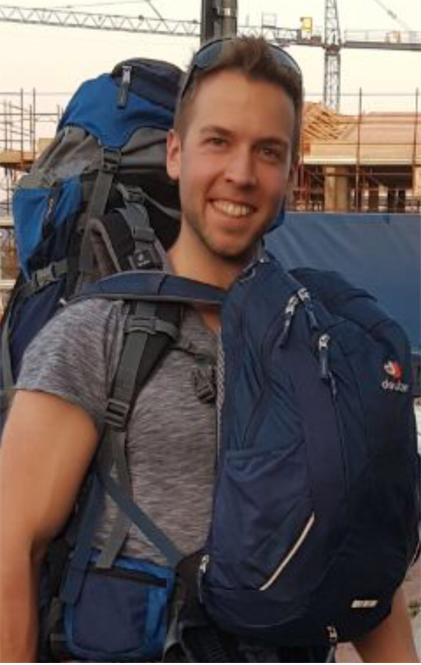
\includegraphics[width=3.3cm]{res/philipp_van_wickevoort_crommelin.PNG}
\end{wrapfigure}
~
"Was machst Du eigentlich nach dem Abi?", unterbrach ich das abwechslungslose Rauschen des 70\,PS schwachen Dieselmotors unseres
VW-Bus-T3s bei 80\,km/h Höchstgeschwindigkeit auf der slowenischen Avtocesta, der Bundesautobahn A2, bei der Durchfahrt im
Karawankentunnel – noch rund 300\,km von unserem Ziel, der kroatischen Halbinsel Istrien, entfernt.
Mich verblüfft heute noch, wie prompt die Antwort kam.

"Physik studieren!", erwiderte mein guter alter Freund Johann und fügte nach kurzer Pause hinzu: "Weil ich dort die Fähigkeit erlerne, logisch zu denken."
Das Selbstverständnis, das in der Betonung seiner Antwort lag, sollte noch viele Jahre in meinem Bewusstsein wiederhallen... \\ 

Rund ein Jahr später besiegelte ich meine schulische Laufbahn mit einem durchschnittlichen bis guten Abitur und entschied daraufhin,
eine Rucksackreise nach Zentralamerika anzutreten.
Dort hatte ich vor allem eines: Zeit. In erster Linie habe ich die dazu genutzt, um meine Reise mit jedem Schritt zu genießen.
Es gab allerdings auch ausreichend Zeit, um etwas mehr über die nächsten, größeren Schritte im Leben zu sinnieren. Johanns Bemerkung fiel mir wieder in den Sinn... \\ 

Physik studieren? Das ist doch nur was für hochbegabte Nerds. Für Außenseiter, die sich während der Schulzeit regelmäßig zu LAN-Parties verabredeten und 
von den \textit{coolen} Jungs kopfüber in die Kloschüssel getaucht wurden -- ein Auffangbecken der personifizierten, sozialen Inkompetenz.
Zu dieser Sorte Jungs habe ich zwar nie gehört, allerdings auch nicht zu den Überfliegern.
"Physik ist die Mutter aller Naturwissenschaften!", erinnerte ich mich an das – zumindest im monatlichen Intervall – gebetsartig aufgesagte Mantra unseres
Physik- und Klassenlehrers. Je mehr ich darüber nachdachte, desto mehr klang es nach Herausforderung,
nach einem Tiefentauchgang in die Welt der Astronomie und der Quanten.
Es klang nach Aussicht auf ein tiefgreifendes Verständnis der uns umgebenden Welt. Ich wollte es versuchen... \\ 

Beim Besuch der ersten Mathe-\textsc{I}-Vorlesung an der \textsc{Christian-Albrechts}-Universität zu Kiel ahnte ich nichts von meinem Glück, dass mir dieses Fach in den kommenden Monaten 90\,\% meiner Kopfschmerzen
verursachen und zeitlichen Kapazitäten abverlangen würde.
Auf die restlichen 10\,\% fielen Physik \textsc{I}, ein Computer-, ein Chemie- und ein weiterer – allerdings etwas angewandterer – Mathe-Grundkurs. \\ 

Ich wollte ihn schon korrigieren... Der Professor musste dem Anschein nach völlig falsch verstanden haben, was \textit{Mathematik} eigentlich war,
nämlich eine Gleichung nach $x$ umzustellen oder mal eine Kurvendiskussion durchzuführen – so hatte man es doch noch aus der Schulzeit in Erinnerung.
Anstelle dessen wurden Axiome, Lemmata, Beweise, Abschätzungen und Grenzgänge allgegenwärtiges Idiom.
Man musste schon aufpassen im privaten Umfeld zu vermeiden, jeden Satz mit "Sei Epsilon größer Null..." anzufangen. \\ 

Ich habe gebüffelt wie verrückt und nach Abschluss der Matheprüfung mit Note 3,7 wurden mir zwei Dinge klar: 1., das Physikstudium ist undankbar aber
machbar – auch als Normalo – und 2., die Regelstudienzeit ist definitiv keine Option - jedenfalls nicht als Normalo.
So wurden aus 6 Semestern 1-Fach-Bachelorstudium am Ende 8, womit für ein Studentenleben außerhalb des
Bibliothekskellers endliche Wahrscheinlichkeiten bestanden. Nach diesen 8 Semestern hatte ich 1., einen 1-Fach-Bachelor der Physik, 2., ein paar Tassen weniger im
Schrank und 3., die Faxen von der Materie erstmal dicke. \\ 

Zur Frage nach dem \textit{nächsten Schritt} war man gar nicht gekommen und plötzlich sah man sich damit konfrontiert.
Wer sich diese Frage stellt, kommt allerdings gleich zur nächsten: "Was, zur Hölle, will ich mit einem Abschluss in Physik?". \\ 

Ich wusste jedenfalls, falls es weitergehen soll, dann musste ein Tapetenwechsel her – andere Stadt, andere Uni, andere Professoren und andere Themen.
Nach einiger Recherche habe ich mich für Münster entschieden – Deutschlands Fahrradhauptstadt.
Das war eine gute Idee, denn in Münster gibt es scheinbar keine Probleme: 

Hoppelnde Karnickel auf Hauptverkehrskreiseln, perfekt begradigte Straßenmarkierungen auf perfekt geteerten Straßen, eine Polizei, die systemgefährdende Über-Rot-Gänger noch zur Rechenschaft zieht, die perfekte Balance zwischen städtischem Erholungs- und Wohnraum, kulturelle Vielseitigkeit für Jung und Alt und ein gefühlt verpflichtender, allsonntäglicher Kirchengang, den erfolgreich zu vermeiden sicherlich kein Problem darstellen würde. Kurzum, Münster war das perfekte Umfeld für ein akademisches Aufbaustudium unter Vermeidung blasphemischer Ablenkungen. \\ 

Wer das Masterstudium dann beginnt, kann sich erstmal zurücklehnen.
Die Vorlesungen können meist aus einem sehr vielfältigen und stark individualisierbaren Studienprogramm zusammengestellt werden. 
Die Tage der großen Vorlesungshörsäle sind gezählt und man sitzt meist nur noch mit wenigen Kommilitonen zusammen und pflegt ein wesentlich
persönlicheres Verhältnis zum Professor.
Wer sich für ein Masterstudium der Physik entscheidet, der beweist nicht zuletzt seine Überzeugung, die er der Sache widmet.
Die Probezeit ist sozusagen vorbei und dieses Gefühl wird einem meist auch von den Dozenten widergespiegelt. \\ 

Die Frage, was ich mit einem Master-Abschluss der Physik eigentlich machen will, war immer noch ungeklärt und so entschied ich mich für ein Praktikum in einer Bank.
Wie ich darauf kam? In Münster kann man sich so ziemlich alles in den Studienplan laden,
so auch das Seminar \textit{Finanzmathematik und Risikomanagement} des theoretischen Kernphysikers \textsc{Dr. Jörg C. Lemm}, das dem Alltag erfrischend abwechslungsreichen Kontrast verpasste. \\ 

Ich kann jedem ein Praktikum nur empfehlen. Nicht zuletzt, weil man als Physikstudent häufig wenig Vorstellung davon hat, was man außerhalb der Uni alles Tolles mit seinem Wissen anfangen kann.
Ich fand die Bankenwelt interessant, insbesondere, weil man dort die erlernte Mathematik und erlernten Programmierkenntnisse einbringen konnte.
Heute arbeite ich für die parcIT GmbH, dem "Partner für Risikomanagement und Controlling".
Meine Arbeit macht mir Spass, ich kann viel programmieren, knifflige Probleme kreativ lösen und habe tolle Kollegen. Warum ich nach meinem Master-Abschluss keine Promotion machen wollte?
Vielleicht kommt die irgendwann noch mal. Lebensläufe sind heutzutage nichtlinear und solche Möglichkeiten bleiben meiner Ansicht nach weiter offen. \\ 

Zum Schluss zurück zu Johanns Aussage. Erlernt man im Physikstudium die Fähigkeit logisch zu denken? Ich denke mittlerweile,
dass ein rationaler Denkapparat eine durchaus gewinnbringende Komponente in der Ausbildung zum Physiker ist. Es geht aber vielmehr darum,
das Handwerkszeug an die Hand zu bekommen, ein komplexes Problem in einfachere, verdaulichere Bausteine zu zerteilen,
die mit mathematischer Logik und den Gesetzen der Natur gelöst werden können.
Es sollte einem klar sein, dass man im Gegensatz zu einem Ingenieur oder einem Architekten keine spezifische Berufsausbildung genießt.
Als Physiker ist man Generalist, der allerdings dazu befähigt ist, sich in jede erdenklich Nische einzuarbeiten und sich auf diese zu spezialisieren. \\ 

Deswegen lautet mein Appell an alle, die noch an der Entscheidung zweifeln: "Traut Euch, denn es lohnt sich!" und alle, die unter dem Druck des Studiums leiden: "Haltet durch, denn es lohnt sich!" Ich für meinen Fall, würde es wieder machen. \\ 

\vspace{0.8cm}

\fibelsig{Philipp van Wickevoort Crommelin}



\end{multicols}
